\documentclass{article}
\usepackage[a4paper,width=150mm,top=25mm,bottom=25mm,bindingoffset=6mm]{geometry}

\usepackage{float}
\usepackage{amsmath}
\usepackage[english]{babel}
\usepackage[utf8x]{inputenc}
\usepackage{graphicx}
\usepackage[colorinlistoftodos]{todonotes}
\usepackage{listings}
\usepackage{color}
\usepackage{multirow}
\newcommand\numberthis{\addtocounter{equation}{1}\tag{\theequation}}

\lstset{
language=R,
basicstyle=\scriptsize\ttfamily,
commentstyle=\ttfamily\color{green},
numbers=left,
numberstyle=\ttfamily\color{blue}\footnotesize,
stepnumber=1,
numbersep=5pt,
backgroundcolor=\color{white},
showspaces=false,
showstringspaces=false,
showtabs=false,
%frame=single,
tabsize=2,
captionpos=b,
breaklines=true,
breakatwhitespace=false,
title=\lstname,
escapeinside={},
keywordstyle={},
morekeywords={}
} 
\usepackage{enumitem}
\usepackage{subcaption}
\usepackage{parskip}

\title{Simulation of Chord Peer-to-peer Network: \\
Distributed System (Graduate Course)}

\author{Chih-Yuan Lin \\
chih-yuan.lin@liu.se \\
Department of Computer and Information Science\\
Linköping University\\}
\begin{document}
\maketitle
\begin{center}
--------------------------------------------------------------------------------\\
\end{center}

\section*{Introduction}
%Write a basic simulator (in the language of your choice) that simulates the Chord peer-to-peer protocol.  
%Your code should support (i) node insertion and (ii) message forwarding.  
%Then, simulate example scenarios and report how the overhead of node insertion and packet forwarding scales with the number of nodes in your Chord implementation.  
%Your report should reflect on your findings and compare with results from the existing literature.
This report summarizes the project work of the Distributed System course. Our assignment was to implement a basic simulator of Chord peer-to-peer network proposed by Stoica et al \cite{paper, report} and measure the overhead of node insertion and message forwarding scales with the number of nodes.

\section*{Implementation}
Our simulator was implemented with Python in an object-oriented manner. A Chord network is maintained by a list of Node instances. Messages are forwarded as arguments between public methods of two instances (i.e, without passing through RPC). Fig. \ref{node} shows the class variables and methods. 

In this project, we implement a simple Chord-based lookup service. Each Chord node has a variable \textit{ip} keeping its IP address and an \textit{ID\_LEN}-long \textit{id} which is produced by hashing the IP address with SHA-1 function. To improve the scalability, Chord protocol requires more routing information than just a successor pointer. Variable \textit{predecessor} is the predecessor pointer and \textit{fingers} is the finger table. The finger table contains \textit{ID\_LEN} entries. The $i^{th}$ entry of node $n$ stores the pointer of the first node, $s$, that succeeds $n$ by at least $2^i$, where $1 \leq i \leq m$. Last, we implement the storage with the build-in dictionary data type, that stores pairs of strings and secret numbers. The details and pseudo code of the other methods can be found in the original paper.
\begin{figure}[H]
\centering
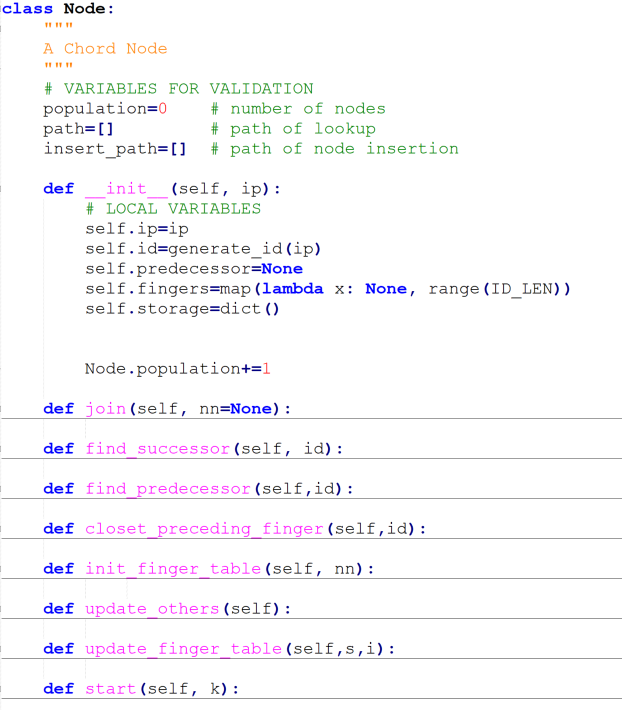
\includegraphics[scale=1.5]{Node.PNG}
\caption{The Node class.
\label{node}}
\end{figure}

We also provide three APIs to manipulate the Chord network as shown in Fig. \ref{api}
\begin{enumerate}
\item Key location
\item Lookup
\item Node insertion
\end{enumerate}
We test only the Lookup and Node insertion as required.
\begin{figure}[H]
\centering
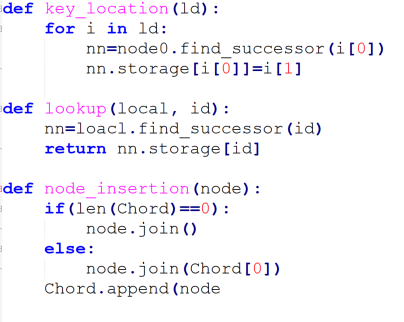
\includegraphics[scale=1.5]{APIs.PNG}
\caption{The defined APIs
\label{api}}
\end{figure}

\section*{Performance}
This section describes how we measure the overhead of node insertion and message forwarding and the resulting performance.
\subsection*{Experiment Settings}
\textbf{Message forwarding.} Message forwarding in a Chord network is triggered by a lookup operation. The original paper evaluates the lookup performance with the metric path length, which is defined as the number of nodes traversed during a lookup operation. The paper presents the path length in a network that contains $2^k$ random nodes and $100 \times 2^k$ random keys in all. It varies the $k$ from $3$ to $14$ and conducts an separate experiment for each $k$. Each node in each experiment picked a random set of keys to query from the system, and it measures the path length required to resolve each query on average. In order to compare our work with the original paper, we follow the same settings of experiments.


\textbf{Node insertion.} Node insertion performance is not tested in the original paper. Thus, we extend the definition of path length here. We measure the number of nodes traversed during \textit{init\_finger\_table} and \textit{update\_finger\_table} and refer to this measurement as path length of node insertion. Our experiments to measure the overhead of node insertion are conducted in the same Chord networks as the above. For each experiment, we insert a random node into a $2^k$ random network. We repeats the experiment $20$ times for each $k$.

\subsection*{Results}
Fig. \ref{lookup} presents the median, $1^{st}$, and $99^{th}$ percentiles of path length of lookup as a function of $k$. The red line is generated by $\frac{1}{2}logN$. We can see that the path length increases logarithmically as proposed. Compare to the proposed performance in Fig. \ref{oldlookup}, the length of routing path is quite similar. 
\begin{figure}[H]
\centering
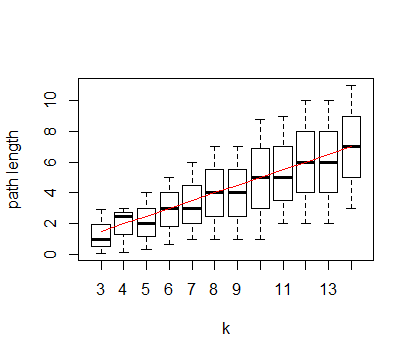
\includegraphics[scale=1.2]{lookup.png}
\caption{The path length of lookup operation as a function of $k$.
\label{lookup}}
\end{figure}

\begin{figure}[H]
\centering
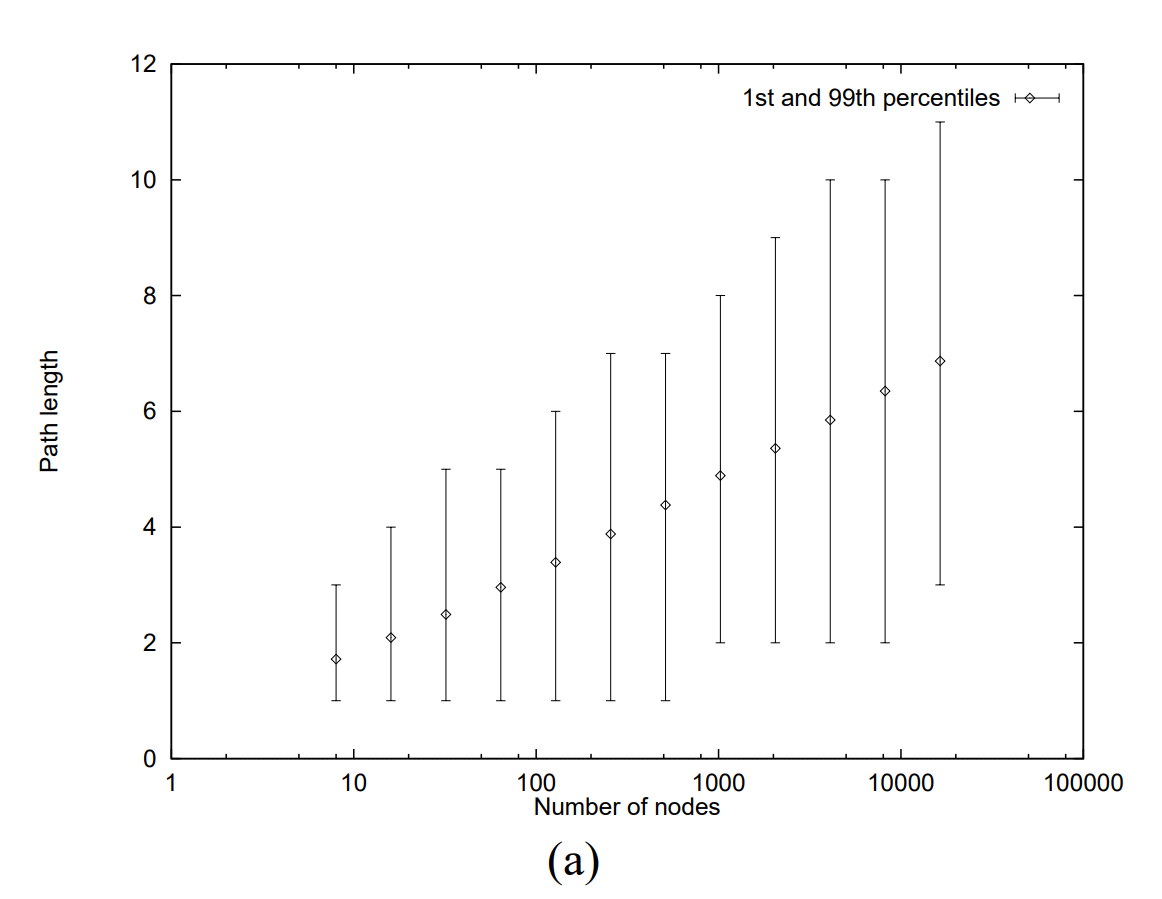
\includegraphics[scale=1]{oldlookup.PNG}
\caption{The path length of lookup operation as a function of network size.
\label{oldlookup}}
\end{figure}

Fig.\ref{insert} shows the median, $1^{st}$, and $99^{th}$ percentiles of path length of node insertion as a function of $k$. The red line is generated by $ZlogN$, where $Z \propto ID\_LEN$ and has to be determined experimentally. In our experiments, $Z=135$ when $ID\_LEN=160$ and $Z=70$ when $ID\_LEN=80$.

\begin{figure}[H]
\centering
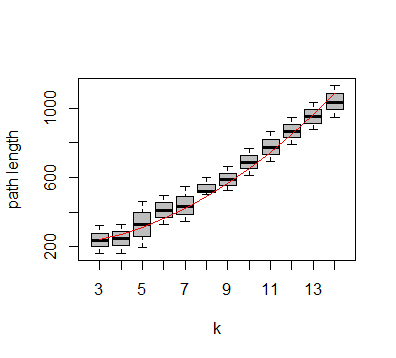
\includegraphics[scale=1.2]{insertion.png}
\caption{The path length of node insertion as a function of $k$
\label{insert}}
\end{figure}


%\begin{equation}
%K(u)=exp(-\parallel u \parallel^2).
%\end{equation}



\bibliographystyle{unsrt}
\bibliography{refs}

\end{document}



